\documentclass{article}
\usepackage{physics}
\usepackage{amsmath}
\usepackage{amsfonts}
\usepackage{amsthm}

\usepackage{float}
\usepackage{graphicx}

\newtheorem{fact}{Fact}
\newtheorem{definition}{Definition}
\newtheorem{problem}{Problem}
\newtheorem{lemma}{Lemma}
\newtheorem{theorem}{Theorem}

\DeclareMathOperator{\dist}{dist}
\DeclareMathOperator{\length}{length}
\title{The Summary of Findings}
\author{Seyed Sajad Kahani}
\date{July 2021}
\begin{document}
\maketitle
\section{Results}
\subsection{No-go theorem for speedup in PIP}
\begin{problem}[\textsc{Point-In-Polygon}]
\label{problem:pip}
Given a point $p \in \mathbb{R}^2$ and a polygon with $n$ points named  $q_1, \dots, q_n \in \mathbb{R}^2$, we say \textsc{Yes} if $p$ lies inside the polygon and \textsc{No} otherwise. 
\end{problem}

\begin{theorem}
\label{theorem:quantum-nogo}
Quantum query complexity of problem \ref{problem:pip} is $\Omega(n)$.
\end{theorem}

\begin{fact}
There is a classical algorithm that can solve problem \ref{problem:pip} using $\Theta(n)$ queries in $\Theta(n)$ time.
\end{fact}

\subsection{Superpolynomial speedup in PIPP}

\begin{problem}[\textsc{Point-In-Polygon-Promise}]
\label{problem:pipp}
Same as problem \ref{problem:pip}, but it's promised that the apparent angle $\theta_i$ of each edge $e_i := (q_i, q_{i+1})$ from the viewpoint of $p$ is less than $\frac{2\pi\kappa}{n}$, where $\kappa$ is an $O(1)$ constant.
\end{problem}

\begin{theorem}
\label{theorem:classical-nogo}
Classical query complexity for any bounded-error deterministic algorithm that solves problem \ref{problem:pipp} is $\omega(1)$.
\end{theorem}

\begin{theorem}
\label{theorem:quantum-algorithm}
There is a bounded-error quantum algorithm that can solve problem \ref{problem:pipp} using $\Theta(1)$ queries in $\Theta(\log(n))$ time.

\begin{equation}
    \begin{cases}    
    \Pr(\text{\textsc{Yes}} | \text{in}) = \frac{1}{\kappa^2} \\
    \Pr(\text{\textsc{No}} | \text{out}) = 1 \\
    \end{cases}
\end{equation} 

\end{theorem}

\section{Proofs}
\begin{problem}[\textsc{Parity}]
\label{problem:parity}
Given a bitstring consisting of $n$ bits, we say \textsc{Yes} if the hamming weight of the bitstring is even, otherwise \textsc{No}.
\end{problem}

\begin{lemma}
\label{lemma:reduction}
Problem \ref{problem:parity} can be reduced to problem \ref{problem:pip} with no query overhead.
\end{lemma}
\begin{proof}
Assume a regular polygon with $n$ points $q_1, \dots, q_n$, naming its center point $p$. We can map each point to each bit. If the bit is equal to $1$, we reflect $q_i$ and then scale by $\alpha \ne 1$ with respect to $p$.

Now, solving problem \ref{problem:pip} for the polygon will solve problem \ref{problem:parity}. Note that for each point query, we need to do exactly $1$ bit query. 
\end{proof}

\begin{proof}[Proof of theorem \ref{theorem:quantum-nogo}]
First, We prove a lower bound for problem \ref{problem:parity}. Using quantum adversary bound \cite{ambainis2002}, we can create a hypercube associated with the bitstring that can be seen as a bipartite that one part is the set of bitstrings with output \textsc{Yes} in problem \ref{problem:parity} and the other part with \textsc{No}. The degree of nodes is equal to $n$ on each part, and defining subgraphs $G_i$ for edges associated with $i$-th bitflip, they'll have node with degree equal to $1$.

Then the lower bound will be 
\[ \Omega\left(\sqrt{\frac{mm'}{ll'}}\right) = \Omega(N) \]

We can use lemma \ref{lemma:reduction} to generalize the lower bound to problem \ref{problem:pip}.
\end{proof} 

\begin{definition}
\label{def:cresent}
Assume a regular polygon with $n$ points and a center called $p$. We define cresent transformation as if we transform $k \le n/2$ sequential edges to make a cresent shape and make $p$ out of the polygon. It's easy to show that $\kappa = \max \theta_i$ (as it's defined in \ref{problem:pipp}) in this transformation will change from $1$ to $\frac{n-k}{k}$
\end{definition}

\begin{figure}[H]
\centering
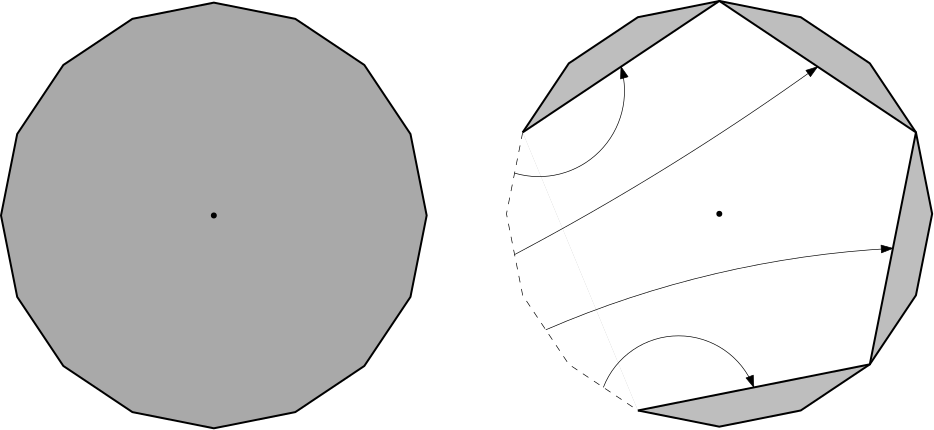
\includegraphics[width=0.8\textwidth]{shape.png}
\caption{Illustration of lemma \ref{def:cresent}}
\end{figure}

\begin{proof}[Proof of theorem \ref{theorem:classical-nogo}]
Assume a regular polygon with $n$ points and a center called $p$ (as in definition \ref{def:cresent}). If we use $t$ queries, where $t \in \Theta(1)$, there are $\lceil\frac{n - t}{t}\rceil + 1 \in \Theta(n)$ sequential edges are left in between. These edges are totally unkown (note that two ends are fixed).
Then we can apply cresent transformation on the sequential edges that results in a new polygon, that the following statements are all true for them.
\begin{itemize}
    \item The old one and the new one cannot be distinguished with those queries.
    \item The promise $k \in O(1)$ is valid for both polygons.
    \item The result of problem \ref{problem:pipp} differs for these two polygons.
\end{itemize}
This means that $t$ queries aren't sufficient to solve this problem and we need $t \in \omega(1)$ queries. 
\end{proof}

\begin{proof}[Proof of theorem \ref{theorem:quantum-algorithm}]
This algorithm is completely studied in the thesis, but the proof sketch is to compute winding number \cite{hormann} using quantum Hadamard transform which is similar to Duetch-Joza algorithm\cite{deutsch}.
\end{proof}

\bibliography{refs.bib}
\bibliographystyle{plain}
\end{document}
